\section{Three Parameter Solar Cell Model}\label{sec:three_parameter_solar_cell_model}

\subsection{Model Introduction}\label{subsec:three_param_model_introduction}

\begin{figure}[h]
    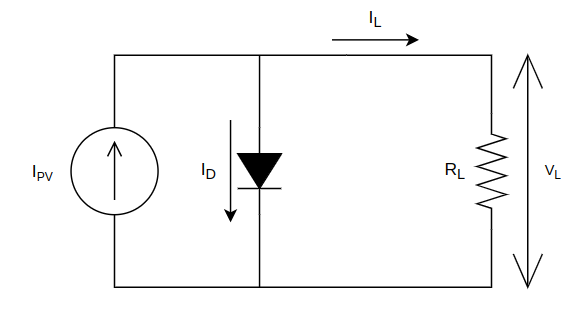
\includegraphics[width=\textwidth]{solar_cell_three_parameter_model.png}
    \caption{Three Parameter, or Single Diode Model of a Solar Cell}
    \label{fig:single_diode_model}
\end{figure}

The most basic model of a solar cell is the three parameter model, or single
diode model, shown in \autoref{fig:single_diode_model}. It consists of a
constant current source and a diode. The constant current source produces a
\ac{IPV} caused by photons of sufficient energy being absorbed into the surface
of the solar cell and exciting charge carriers (generally in the form of
electrons) to enter the circuit. The diode represents the various recombination
processes that consume the generated current in the form of \ac{ID}.

In this model, the three parameters consist of the following:

\begin{itemize}
    \item \acf{IPV},
    \item \acf{I0},
    \item and an \acf{N}.
\end{itemize}

The latter two are contained within the dark current term, and generally
influence the shape of the predicted \ac{I-V} curve, particularly around the
knee-bend.

This model is juxtaposed from the five parameter model in that it does not
incorporate cell losses in the form of \ac{RS} and \ac{RSH}. It is assumed that
in this model, the series resistance is zero (short circuit) and the shunt
resistance is infinite (open circuit). Therefore, the five parameter model may
also be called the complete single diode model.

We observe from \autoref{fig:single_diode_model} that the \ac{IL} can be
represented as a function of the photocurrent and the dark current, shown in
\autoref{eq:cell_output_current_1}.

\begin{equation}
    I_L = I_{PV} - I_D
    \equnit{\si{\ampere}}
    \label{eq:cell_output_current_1}
\end{equation}

In the following subsections, we break down each component into its constituent
parts.


\subsection{Photocurrent}\label{subsec:three_param_photocurrent}

\begin{equation}
    I_{PV} = qA\int_{}{}b_s(E)QE(E)dE
    \equnit{\si{\ampere}}
    \label{eq:cell_photocurrent_1}
\end{equation}

On a fundamental level, we can define the \acf{IPV} as a function of the photons
incident upon the surface of the solar cell and the solar cell's spectral
response. This is demonstrated in \autoref{eq:cell_photocurrent_1}. A bulleted,
simplistic explanation of this equation is presented as follows:

\begin{itemize}
    \item Incident light hits the solar cell over a given spectrum of energy
    levels (denoted either in $eV$ or in $nm$) (see
    \autoref{fig:maxeon_gen_iii_cell_spectral_response}).
    \item Incident light at each discrete energy level has an \ac{BS}, otherwise
    known as intensity.
    \item The solar cell has a given \ac{QE} at each energy level that is the
    probability that an incident photon of \ac{E} delivers one electron to the
    external circuit.
    \item Integrating the product of the photon flux density \ac{BS} and quantum
    efficiency \ac{QE} (then multiplied by the \ac{Q} and the cell \ac{A})
    provides the photocurrent (\ac{IPV}).
\end{itemize}

\begin{figure}[h]
    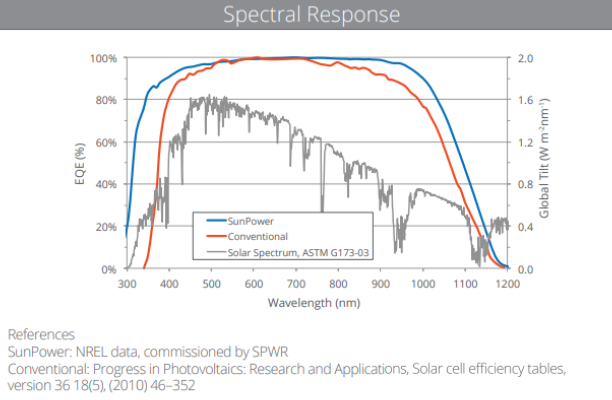
\includegraphics[width=\textwidth]{maxeon_gen_iii_cell_spectral_response.png}
    \caption{Maxeon Gen III Cell Spectral Response}
    \label{fig:maxeon_gen_iii_cell_spectral_response}
\end{figure}

Solar cell manufacturers may provide a spectral response chart showing the
quantum efficiency over the useful solar spectrum (as seen in
\autoref{fig:maxeon_gen_iii_cell_spectral_response}), but will generally just
provide the \ac{ISC} at \ac{STC} ($1000$ $Wm^{-2}$, $AM$ $1.5G$, $25$ $C$).

As it turns out, the photocurrent can generally be approximated as the short
circuit current. We'll discuss in \autoref{subsec:five_param_series_resistance}
that Cubas et al.~\cite{cubas_et_al}\cite{cubas_et_al_2} defines the
photocurrent as a ratio of the series and shunt resistance in addition to the
short circuit current. However, in most cases, the empirical value of \acl{ISC}
will not differ from \autoref{eq:cell_photocurrent_2}.

\begin{equation}
    I_{PV} = I_{SC}
    \equnit{\si{\ampere}}
    \label{eq:cell_photocurrent_2}
\end{equation}


\subsection{Dark Current}\label{subsec:three_param_dark_current}

The \acf{ID} comprises of the interesting and critical parameters of the three
parameter model; shown in \autoref{eq:cell_dark_current_1}, it consists of the
term \ac{I0} and an exponential. The exponential is a function of three key
variables: the \acf{TC}, \acf{VL}, and \acf{N}.

\begin{equation}
    I_D = I_0[\exp(\frac{V}{V_T}) - 1]
    \equnit{\si{\ampere}}
    \label{eq:cell_dark_current_1}
\end{equation}

This ideality factor is typically between $1$ and $2$, and represents the
proportional influence of carriers inbseveral recombination processes for a
given cell composition and structure. Some ideality factor values are presented
in \autoref{table:ideality_factors}, sourced from PVEducation's Ideality Factor
page~\cite{pveducation_ideality_factor}. We note that the ideality factor may be
outside the typical range of $[1, 2]$, as discussed by Jain et
Kapoor~\cite{jain_et_kapoor} and R.N. Hall~\cite{hall}, the latter of which
notes that auger recombination dominated dark currents may generate a \ac{N} of
$2/3$.

The term \ac{VT} (\autoref{eq:cell_thermal_voltage}) which encapsulates the cell
temperature dependency describes the voltage across the P-N junction of the
diode in the model: at \ac{STC} this is typically $26$ $mV$.

\begin{equation}
    V_T = \frac{n k_B T_C}{q}
    \equnit{\si{\volt}}
    \label{eq:cell_thermal_voltage}
\end{equation}

\begin{table}[h!]
    \begin{tabularx}{\textwidth}{
        | >{\raggedright\arraybackslash}X
        | >{\raggedright\arraybackslash}X
        | >{\raggedright\arraybackslash}X | }
        \hline
        Recombination Type & Ideality Factor & Description \\ \hline \hline
        SRH, band to band (low level injection) & 1 & Recombination limited by minority carrier. \\ \hline
        SRH, band to band (high level injection) & 2 & Recombination limited by both carrier types. \\ \hline
        Auger & 2/3 & Two majority and one minority carriers required for recombination. \\ \hline
        Depletion region (junction) & 2 & Two carriers limit recombination. \\ \hline
    \end{tabularx}
    \caption{Various Ideality Factors of \ac{N}}
    \label{table:ideality_factors}
\end{table}


\subsection{Dark Saturation Current}\label{subsec:three_param_dark_sat_current}

The \acf{I0} has two potential derivations. Generally, the three parameter
model, (see Baig et al.~\cite{baig_et_al}, MacAlpine et
Brandemuehl~\cite{macalpine_et_brandemuehl}, Rusirawan et
Farkas~\cite{rusirawan_et_farkas}, and others) define \ac{I0} as in
\autoref{eq:cell_dark_sat_current_1}; where the diode current is a function of
the cell temperature and the energy bandgap in relation to several reference
parameters at \ac{STC}.

\begin{equation}
    I_0 = I_{0,ref}{(\frac{T_C}{T_{C,ref}})}^3\exp(\frac{E_{G,ref}}{k_B T_{C,ref}} - \frac{E_G}{k_B T_C})
    \equnit{\si{\ampere}}
    \label{eq:cell_dark_sat_current_1}
\end{equation}

On the other hand, we can derive the \ac{I0} algebraically: given the short
\acf{ISC} and \ac{VOC}, we can set the cell at open circuit,
forming the derivation in \autoref{eq:cell_dark_sat_current_deriv} and the
result in \autoref{eq:cell_dark_sat_current_2}.

\begin{equation}
    \begin{split}
        I_L &= 0 \\
        & = I_{SC} - I_D \\
        & = I_{SC} - I_0[\exp(\frac{V_{OC}}{V_T}) - 1]
    \end{split}
    \equnit{\si{\ampere}}
    \label{eq:cell_dark_sat_current_deriv}
\end{equation}

\begin{equation}
    I_0 = I_{SC}[\exp(\frac{V_{OC}}{V_T}) - 1]^{-1}
    \equnit{\si{\ampere}}
    \label{eq:cell_dark_sat_current_2}
\end{equation}

The latter model is convenient since it does not require measuring \ac{I0REF},
\ac{EGREF}, nor \ac{EG}. As such, we will only evaluate the latter model in
\autoref{sec:evaluation_of_solar_cell_models}.


\subsection{Short Circuit Current}\label{subsec:three_param_short_circuit_current}

Finally, for the three parameter model, we derive the dependence of \acf{ISC}
and \acf{VOC} on \acf{G} and \acf{TC} before establishing the final derivation
of \autoref{eq:cell_output_current_1}.

Starting with the \acf{ISC}, it is known that there is a large positive
correlation with irradiance and a small positive correlation with temperature,
shown in \autoref{fig:cell_temperature_dependence} and
\autoref{fig:cell_irradiance_dependence}.

\begin{figure}[!htbp]
    \centering
    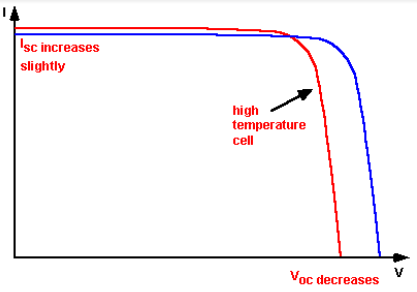
\includegraphics[width=0.7\linewidth]{cell_temperature_dependence.png}
    \caption{Solar Cell Temperature Dependence}
    \label{fig:cell_temperature_dependence}
\end{figure}

\begin{figure}[!htbp]
    \centering
    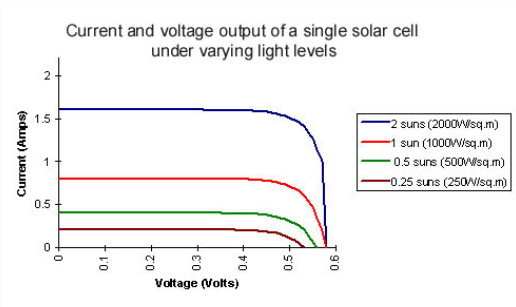
\includegraphics[width=0.9\linewidth]{cell_irradiance_dependence.png}
    \caption{Solar Cell Irradiance Dependence}
    \label{fig:cell_irradiance_dependence}
\end{figure}

The dependence of irradiance on $I_{SC}$ can be modeled as linearly proportional
to the light incident upon the solar cell over the reference irradiance. This
makes intuitive sense: given half the available light (assuming the distribution
of light across the spectrum is consistent), the solar cell will only be able to
capture half the maximum available power. Chegaar et al.~\cite{chegaar_et_al}
proposes this relationship as \autoref{eq:cell_short_circuit_current_1}, where
the short circuit current is a function of \ac{KE} and \acf{G} (the latter in
units of $Wm^{-2}$).

\begin{equation}
    I_{SC}(G) = K_E G
    \equnit{\si{\ampere}}
    \label{eq:cell_short_circuit_current_1}
\end{equation}

\autoref{eq:cell_short_circuit_current_1} can be easily reworked where the
constant \ac{KE} is now based on a \acf{ISCREF} and a \ac{GREF}. This forms
\autoref{eq:cell_short_circuit_current_2}, which is the same form used by Baig
et al.~\cite{baig_et_al}.

\begin{equation}
    I_{SC}(G) = I_{SC,ref}\frac{G}{G_{ref}}
    \equnit{\si{\ampere}}
    \label{eq:cell_short_circuit_current_2}
\end{equation}

Hishikawa et al.~\cite{hishikawa_et_al} proposes modeling the dependence of
temperature on \ac{ISC} using a \acf{ALPHA}
(\autoref{eq:thermal_coefficient_alpha}). \ac{ALPHA} is empirically determined
and varies given the material composition and structure of the solar cell; for
crystalline silicon solar cells, this is approximately 0.05\%/K, or 0.0005.
\autoref{eq:thermal_coefficient_alpha} can be rearranged to form
\autoref{eq:cell_short_circuit_current_3}. This is effectively equivalent to
Rusirawan et Farkas~\cite{rusirawan_et_farkas}, but is slightly different from
MacAlpine et Brandemuehl~\cite{macalpine_et_brandemuehl} and Baig et
al.~\cite{baig_et_al}, who take the constant term $1$ and replace it with a
another constant, \ac{ISCREF} (\autoref{eq:cell_short_circuit_current_4}).

\begin{equation}
    \alpha = \frac{1}{I_{SC,ref}}\frac{\Delta I_{SC}}{\Delta T_C} = \frac{1}{I_{SC,ref}}\frac{I_{SC,ref} - I_{SC}}{T_{C,ref} - T_C}
    \equnit{\si{unitless}}
    \label{eq:thermal_coefficient_alpha}
\end{equation}

\begin{equation}
    I_{SC}(T_C) = I_{SC,ref}[1 - \alpha(T_{C,ref} - T_C)]
    \equnit{\si{\ampere}}
    \label{eq:cell_short_circuit_current_3}
\end{equation}

% NOTE: Rusirawan et Farkas derivation to match short_circuit_current_3.
% \begin{equation}
%     \mu = \frac{I_{SC} - I_{SC,ref}}{T_C - T_{C,ref}} = -\alpha I_{SC,ref}
%     \equnit{\si{unitless}}
% \end{equation}
% \begin{equation}
%     I_{SC}(T_C) = I_{SC,ref}+\mu(T_{C,ref} - T_C), where
%     \equnit{\si{\ampere}}
%     \label{eq:cell_short_circuit_current_4}
% \end{equation}

\begin{equation}
    I_{SC}(T_C) = I_{SC,ref}[I_{SC,ref} - \alpha(T_{C,ref} - T_C)]
    \equnit{\si{\ampere}}
    \label{eq:cell_short_circuit_current_4}
\end{equation}

These two competing models of the short circuit current will also be explored
further in \autoref{sec:evaluation_of_solar_cell_models}. For the purposes of
this subsection, however, we will combine
\autoref{eq:cell_short_circuit_current_2} and
\autoref{eq:cell_short_circuit_current_3} to give us
\autoref{eq:cell_short_circuit_current_5}.

\begin{equation}
    I_{SC}(G, T_C) = I_{SC,ref}\frac{G}{G_{ref}}[1 - \alpha(T_{C,ref} - T_C)]
    \equnit{\si{\ampere}}
    \label{eq:cell_short_circuit_current_5}
\end{equation}


\subsection{Open Circuit Voltage}\label{subsec:three_param_open_circuit_voltage}

Likewise, the \acf{VOC} is also a function of temperature and
irradiance. It is known that \ac{VOC} has a medium positive
correlation with irradiance and a medium negative correlation with temperature
(\autoref{fig:cell_temperature_dependence} and
\autoref{fig:cell_irradiance_dependence}).

Returning to \autoref{eq:cell_dark_sat_current_2}, in which we defined the
\acf{I0} as a function of \ac{VOC}, we can invert the equation to retrieve the
\ac{VOC} parameter, shown in \autoref{eq:cell_open_circuit_voltage_1}.

\begin{equation}
    V_{OC} = V_T\ln(\frac{I_{SC}}{I_0} + 1)
    \equnit{\si{\volt}}
    \label{eq:cell_open_circuit_voltage_1}
\end{equation}

There are three points in this equation that can now be determined. We know from
\autoref{eq:cell_thermal_voltage} that the \acf{VT} is dependent on the
\acf{TC}. We can also plug in one of the proposed models for \ac{ISC}. However,
we cannot reuse \autoref{eq:cell_dark_sat_current_2} because
\autoref{eq:cell_open_circuit_voltage_1} was derived from it! Chegaar et
al.~\cite{chegaar_et_al} proposes an alternative form by simplifying the
logarithmic term to form \autoref{eq:cell_open_circuit_voltage_2}.

\begin{equation}
    V_{OC}(G, T_C) = V_{OC,ref} + V_T(T_C)\ln(\frac{G}{G_{ref}} + 1)
    \equnit{\si{\volt}}
    \label{eq:cell_open_circuit_voltage_2}
\end{equation}

This term fits well with the paper’s experimental data, but is not immediately
clear how it models the original term. It also does not properly model
temperature change. \autoref{eq:cell_open_circuit_voltage_3} is a modified
form that implements temperature dependence while retaining irradiance
dependence.

\begin{equation}
    \begin{split}
        V_{OC}(G, T_C) &= V_{OC,ref}[1 - \beta (T_{C,ref} - T_C)] \\
        & \quad+ \frac{nk_B(T_{C,ref} + T_C/\gamma)}{q}\ln(\frac{G}{G_{ref}})
    \end{split}
    \equnit{\si{\volt}}
    \label{eq:cell_open_circuit_voltage_3}
\end{equation}

\begin{equation}
    \beta = \frac{1}{V_{OC,ref}}\frac{\Delta V_{OC}}{\Delta T_C}
          = \frac{1}{V_{OC,ref}}\frac{V_{OC,ref} - V_{OC}}{T_{C,ref} - T_C}
    \equnit{\si{unitless}}
    \label{eq:thermal_coefficient_beta}
\end{equation}

\autoref{eq:cell_open_circuit_voltage_3} implements two changes: a \acf{BETA}
and a \acf{GAMMA}. \ac{BETA} is likewise (to \ac{ALPHA}) empirically determined;
for silicon it known to be -0.3\%/K, or -0.003. \ac{GAMMA} is an experimentally
determined curve fitting term, and may more appropriately model the exponential
decrease of \ac{VOC} at low light conditions. It has an expected operable range
of values between $[1, 100]$, where smaller values correlate to a wider range of
of \ac{VOC} movement at low light conditions. This parameter, however, is not
part of the three parameter cell model. Its efficacy will be explored further in
\autoref{sec:evaluation_of_solar_cell_models}.


\subsection{Model Summary}\label{subsec:three_param_model_summary}

To conclude this section, we will review the components that make up the three
parameter cell model, propose three items of further exploration, and propose a
complete model function that incorporates the topics discussed.

Firstly, the three parameter cell model is composed of a constant current source
and a power consuming diode, representing photogeneration and recombination
effects of the solar cell, respectively. These two components form three
parameters that is the namesake of this section, namely the photocurrent, dark
saturation current, and ideality factor.

Secondly, we explore the construction and interpretation of these three
components, and along the way, examine three areas that deviate from the
existing models that we would like to investigate:

\begin{itemize}
    \item an algebraic derivation of the \acf{I0},
    \item an alternative interpretation of the \acf{ISC} as
    a function of \acf{TC},
    \item and a new \acf{GAMMA} to improve \acf{VOC} modeling at low lighting
    conditions.
\end{itemize}

Finally, we present the complete model and its derivation, in
\autoref{eq:cell_output_current_2}. We observe that this complete model requires
four reference parameters (note that in this paragraph we refer to parameters as
in values that need to be determined and not larger terms used in the naming of
the model):

\begin{itemize}
    \item \acf{GREF}
    \item \acf{TCREF}
    \item \acf{VOCREF}
    \item \acf{ISCREF}
\end{itemize}

and four curve fitting parameters:

\begin{itemize}
    \item \acf{N}
    \item \acf{ALPHA}
    \item \acf{BETA}
    \item \acf{GAMMA}
\end{itemize}

For the cells tested in this project, \ac{ALPHA} and \ac{BETA} were provided
by the manufacturer, Maxeon, but \ac{N} and \ac{GAMMA} were not. Curve fitting
techniques, like simulated annealing, will have to be applied to determine these
two variables, and are explored in
\autoref{sec:evaluation_of_solar_cell_models}.


% TODO: This is equation is a freak of nature... Probably stop at second to last
% step and move most of the derivation to an appendix.
\todo{Reformat this equation}
\begin{equation}
    \begin{split}
        I_L(V_L, G, T_C) &= I_{PV}(G, T_C) - I_D(V_L, G, T_C) \\
        & = I_{SC}(G, T_C) - I_D(V_L, G, T_C) \\
        & = I_{SC}(G, T_C) - I_0[\exp(\frac{V_L}{V_T(T_C)}) - 1] \\
        & = I_{SC}(G, T_C) - I_{SC}(G, T_C)[\exp(\frac{V_{OC}(G, T_C)}{V_T(T_C)}) - 1]^{-1}[\exp(\frac{V_L}{V_T(T_C)}) - 1] \\
        & = I_{SC}(G, T_C) - I_{SC}(G, T_C)\frac{\exp(\frac{V_L}{V_T(T_C)}) - 1}{\exp(\frac{V_{OC}(G, T_C)}{V_T(T_C)}) - 1} \\
        & = I_{SC}(G, T_C) - I_{SC}(G, T_C)\frac{\exp(\frac{qV_L}{n k_B T_C}) - 1}{\exp(\frac{qV_{OC}(G, T_C)}{n k_B T_C}) - 1} \\
        & = I_{SC}(G, T_C)[1 - \frac{\exp(\frac{qV_L}{n k_B T_C}) - 1}{\exp(\frac{qV_{OC}(G, T_C)}{n k_B T_C}) - 1}] \\
        & = I_{SC,ref}\frac{G}{G_{ref}}[1 - \alpha[T_{C,ref} - T_C]][1 - \frac{\exp(\frac{qV_L}{n k_B T_C}) - 1}{\exp(\frac{qV_{OC}(G, T_C)}{n k_B T_C}) - 1}] \\
        & = I_{SC,ref}\frac{G}{G_{ref}}[1 - \alpha[T_{C,ref} - T_C]] \\
        & \quad* [1 + \frac{1 - \exp(\frac{qV_L}{n k_B T_C})}{1 - \exp(\frac{q[V_{OC,ref}[1 - \beta[T_{C,ref} - T_C]] + \frac{nk_B(T_{C,ref} + T_C/\gamma)}{q}\ln(\frac{G}{G_{ref}})]}{n k_B T_C})}] \\
    \end{split}
    \equnit{\si{\ampere}}
    \label{eq:cell_output_current_2}
\end{equation}

\todo[inline]{See \url{https://www.desmos.com/calculator/yp0rhmabkz} to play
around with the complete three parameter solar cell model. Add as a figure later
on compared to experimental data.}
